\subsection{Computation of the \gch}\label{app:gapcost-proof}

In this section we prove (\cref{lem:gapcost}) that we can change the dependency of \GCH on $\gscost$
to $\seedcost$ by introducing a new partial order $\preceq_T$ on the matches.
This way, \cref{lem:computation} applies and we can efficiently compute \GCH.
Recall that the gap-seed cost is ${\gscost = \max(\gapcost,
\seedcost)}$, and that the gap transformation is:

\transformation*

The following lemma allows us to determine whether $\gapcost$ or $\seedcost$
dominates the cost $\gscost$ between two matches, based on the relation
$\preceq_T$.

\begin{lem}\label{lem:transform}%
  Let $u$ and $v$ be two states with $v$ at the start of some seed. Then $u
  \preceq_T v$ if and only if $\gapcost(u,v) \leq \seedcost(u,v)$. Furthermore,~${u \preceq_T v}$ implies $u\preceq v$.
\end{lem}
\begin{proof}
  Let $u = \st ij$ and $v = \st {i'}{j'}$. By definition, $u\preceq_T v$ is equivalent to
  \begin{equation*}
    \begin{cases}
    i {-} j {-} P(u) \leq i' {-} j' {-} P(v)\\
    j {-} i {-} P(u) \leq j' {-} i' {-} P(v)
    \end{cases}\hspace{-1em}\Leftrightarrow
    \begin{cases}
    -\big((i'{-}i)-(j'{-}j)\big) \leq P(u) - P(v)\\
    \phantom{-(}(i'{-}i)-(j'{-}j)\phantom) \leq P(u) - P(v).
    \end{cases}
  \end{equation*}
  This simplifies to
  \begin{equation*}
    \gapcost(u, v) = \abs{(i'-i) - (j'-j)} \leq P(u) - P(v) = \seedcost(u, v),
  \end{equation*}
  where the last equality holds because $v$ is at the start of a seed.

  For the second part, $u\preceq_T v$ implies
  $0\leq \gapcost(u,v)\leq \seedcost(u,v) =  P(u)-P(v)$ and hence
  $P(u) \geq P(v)$. Since $v$ is at the start of a seed, this directly implies
  $i \leq i'$.
  Since seeds have length $k\geq r$ we have
  \begin{equation*}
  \abs{(i'-i) - (j'-j)} \leq P(u)-P(v) = r\cdot \abs{\substr \seeds i{i'}} \leq r\cdot (i'-i)/k \leq i'-i.
  \end{equation*}
  This implies $j'-j\geq 0$ and hence $j\leq j'$, as required.
\end{proof}

A direct corollary is that for $u\preceq v$ with $v$ at the start of some seed, we
have
\begin{equation}
  \gscost(u,v) =
  \begin{cases}
    \seedcost(u,v) & \text{if $u\preceq_T v$,}\\
    \gapcost(u,v) & \text{if $u\npreceq_T v$.}
\end{cases}
\label{eq:trans}
\end{equation}

A second corollary is that ${\start(m) \preceq_T \matchend(m)}$ for all matches
$m {\in} \matches$, since a match from $u$ to $v$ satisfies
$\gapcost(u,v) < r = \seedcost(u,v)$ by definition.

% TRANSFORMED CHAINS

\begin{lem}\label{lem:tchain} %
  When the set of matches $\matches$ is consistent, $\hgchM(u)$ can be computed
  using \mbox{$\preceq_T$-chains} only:
  \begin{equation*}
    \hgchM(u)
    := h^\matches_{\preceq,\gscost}\!(u)
      = \begin{cases}
           h^\matches_{\preceq_T,\gscost}\!(u) & \text{if $u \preceq_T v_t$,} \\
           \gapcost(u, v_t) & \text{if $u\npreceq_T v_t$.}
         \end{cases}
    \label{eq:tchain}
  \end{equation*}
\end{lem}

\begin{proof}
  We write $h:=\hgchM = h^\matches_{\preceq,\gscost}\!$ (\cref{dfn:h}) and $h':=
  h^\matches_{\preceq_T,\gscost}\!$.

  \underline{Case 1: $u\npreceq_T v_t$.}
  Let $u\preceq m_1 \preceq \dots \preceq m_l \preceq v_t$ be a chain minimizing $h(u)$ in
  \cref{dfn:h}, so
  \begin{equation*}
   h(u) = \gscost(u, m_1) + \matchcost(m_1) + \gscost(m_1, m_2) + \dots + \gscost(m_l, v_t).
  \end{equation*}
  By definition, $\gscost \geq \gapcost$, and $\matchcost(m_i) \geq
  \gapcost(\matchstart(m_i), \matchend(m_i))$, so the weak triangle
  inequality~(\cref{lem:weaktriangle}) for $\gapcost$ gives
  \begin{equation*}
   h(u) \geq \gapcost(u, m_1) + \gapcost(m_1) + \dots + \gapcost(m_l, v_t) \geq \gapcost(u, v_t).
  \end{equation*}
  Since $u {\npreceq_T} v_t$, the empty chain $u {\preceq} v_t$ has cost $h(u)
  \leq \gscost(u, v_t) = \gapcost(u, v_t)$. Combining the two inequalities, $h(u) = \gapcost(u, v_t)$.

\begin{figure}[H]
    \centering
    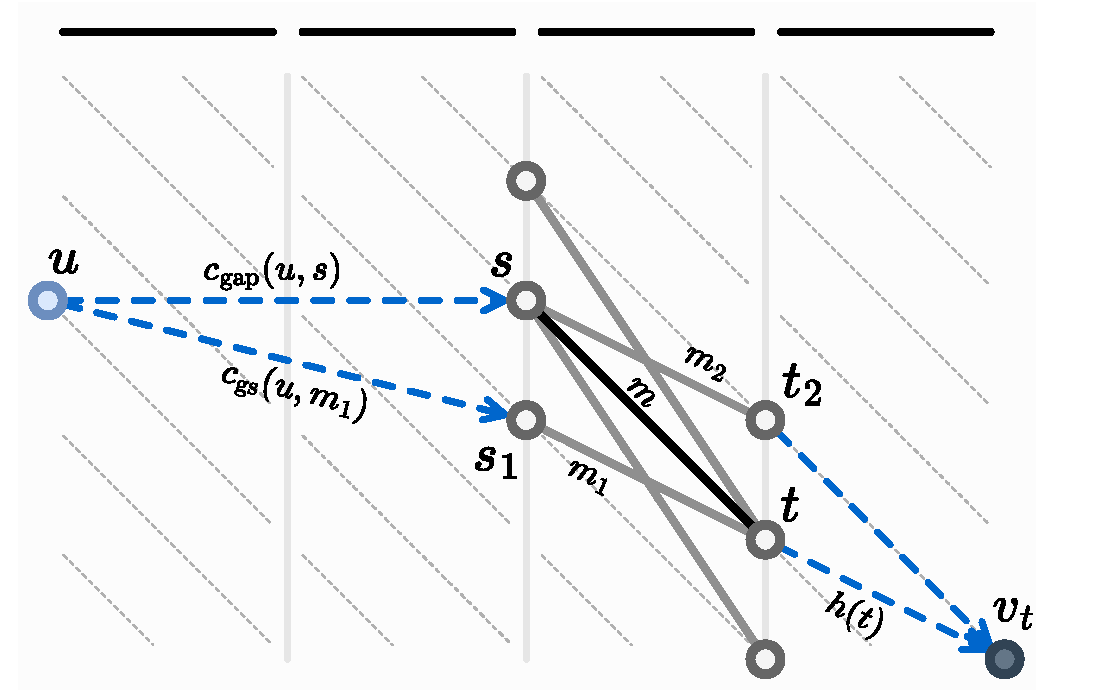
\includegraphics[width=0.7\linewidth]{imgs/proofs/gch-proof.pdf}%
    \caption[Variables in Case 2 of the proof of
      \cref{lem:tchain}]{\textbf{Variables in Case 2 of the proof of
      \cref{lem:tchain}.} Match $m$ has ${\matchscore(m) = 2}$, so it has
      adjacent matches $m_1$ and $m_2$ (\textcolor{gray}{gray}) with
      $\matchscore(m_i) \geq 1$.}
    \label{fig:gch-proof}
\end{figure}

  \underline{Case 2: $u\preceq_T v_t$.} First rewrite $h$ and $h'$ recursively as
  \begin{align}
    \phantom'h(u) &= \min_{\substack{m\in \matches \\ \mathclap{u\preceq m\preceq v_t}}} \big(\gscost(u, m) + \matchcost(m) + \phantom'h(\matchend(m))\big)
    \label{eq:recursion}\\
    h'(u) &= \min_{\substack{m\in \matches \\ \mathclap{u\preceq_T m\preceq_T v_t}}} \big(\gscost(u, m) + \matchcost(m) + h'(\matchend(m))\big),
    \label{eq:recursion2}
  \end{align}
  both with base case $h(v_t){=}h'(v_t)= 0$ after eventually taking $m_\omega$. We will show that
  \begin{equation}
    h(u) = \min_{\substack{m\in \matches\\\mathclap{u\preceq_T m \preceq_T v_t}}} \big(\gscost(u, m) + \matchcost(m) + h(\matchend(m))\big),
    \label{eq:trecursion}
  \end{equation}
  which is exactly the recursion for $h'$, so that by induction $h(u) = h'(u)$.

  By \cref{lem:transform}, every $\preceq_T$-chain is a $\preceq$-chain, so
  $h(u) \leq h'(u)$. To prove $h(u) {=} h'(u)$, it remains to show the reverse
  inequality, $h'(u) \leq h(u)$. To this end, choose a match $m$ that
  \begin{description}%[\quad (priority 0)]
    \item[(priority 0)] minimizes $h(u)$ in \cref{eq:recursion}, and among those, has
    \item[(priority 1)] maximal $\seedcost(u, m)$, and among those, has
    \item[(priority 2)] minimal $\gapcost(u, m)$, and among those, has
    \item[(priority 3)] minimal $\gapcost(m, v_t)$.
  \end{description}
  We show that $u\preceq_T m$~(in 2.A) and $m\preceq_T v_t$~(in 2.B), which
  proves~\cref{eq:trecursion}.

  \underline{Part 2.A: $u\preceq_T m$.}
  Let $s$ and $t$ be the begin and end of $m$~(\cref{fig:gch-proof}),
  and let $m'$ be a match minimizing $h(t)$ in \cref{eq:recursion} so
  \begin{equation*}
  h(t) = \gscost(t, m') + \matchcost(m') + h(\matchend(m')).
  \end{equation*}
  Since $m'$ comes after $t$ we have ${\seedcost(u, m') > \seedcost(u, m)}$
  (p.1) and hence $m'$ does not minimize $h(u)$ (p.0):
  \begin{equation*}
    h(u) < \gscost(u, m') + \matchcost(m') +  h(\matchend(m')).
  \end{equation*}
  Using the minimality of $m$, the non-minimality of $m'$, and the triangle inequality we get
  \begin{align*}
    \gscost(u, s) &+ \matchcost(m) + h(t) = h(u)\\
    & < \gscost(u, m') \hspace{4.5em}+ \matchcost(m') +  h(\matchend(m'))\\
    &\leq \gscost(u, t) + \gscost(t, m') + \matchcost(m') + h(\matchend(m'))\\
    &= \gscost(u, t) + h(t)
  \end{align*}
  so we have
  \begin{equation}
  \gscost(u, m) + \matchcost(m) < \gscost(u, t).\label{eq:minh}
  \end{equation}

  From the triangle inequality for $\gapcost$, from $\gapcost(u, s) \leq
  \gscost(u, s)$, and from $\gapcost(s, t) \leq \matchcost(m)$, and
  from~\cref{eq:minh} we obtain
  \begin{equation*}
    \gapcost(u, t)
    \leq \gapcost(u, s) + \gapcost(s, t)
    \leq \gscost(u, s) + \matchcost(m)
    < \gscost(u, t).
  \end{equation*}
  This implies $\gscost(u, t) = \seedcost(u,t)$ and hence reusing \cref{eq:minh}
  \begin{align*}
    \gapcost(u, s) + \matchcost(m)
    &\leq \gscost(u, s) + \matchcost(m)\\
    &< \seedcost(u, t)
    = \seedcost(u, s) + \seedcost(s, t).
  \end{align*}
  We have $\matchcost(m) = \seedcost(s, t) - \matchscore(m)$, so the above
  simplifies to $\gapcost(u, s) < \seedcost(u, s) + \matchscore(m)$ and since
  these are integers $\gapcost(u, s) \leq \seedcost(u, s) + \matchscore(m) - 1$.

  When $\matchscore(m) = 1$, this implies $\gapcost(u, s) \leq \seedcost(u, s)$
  and $u\preceq_T s = \matchstart(m)$ by \cref{lem:transform}.

  When $\matchscore(m) > 1$, suppose that $\gapcost(u, s) > \seedcost(u,s)\geq
  0$. That means that $u$ is either above or below the diagonal of $s$. Let ${s_1
  = \st{s_i}{s_j \pm 1}}$ be the state adjacent to $s$ on the same side of this
  diagonal as $u$. This state exists since $u\preceq s_1 \preceq t$.
  Then $\gapcost(u, s_1) = \gapcost(u, s) {-} 1$, and by
  consistency of $\matches$ there is a match $m_1$ from $s_1$ to $t$ with
  $\matchcost(m_1) \leq \matchcost(m){+}1$. Then
  \begin{align*}
    \gscost(u, s_1) &+ \matchcost(m_1) +h(t)\\
    \leq \gscost(u, s){-}1 &+ \matchcost(m){+}1 +h(t) = h(u),
  \end{align*}
  showing that $m_1$ minimizes $h(u)$ (p.0). Also $\seedcost(u, m_1) =
  \seedcost(u, m_1)$ (p.1) and $\gapcost(u, m_1) < \gapcost(u, m)$ (p.2), so
  that $m_1$ contradicts the minimality of $m$. Thus, $\gapcost(u, s) >
  \seedcost(u,s)$ is impossible and $u\preceq_T s$.

  \underline{Part 2.B: $m\preceq_T v_t$.}
  When there is some match $m'$ succeeding $m$ in the chain, we have $m\preceq
  m'\preceq v_t$ and hence $m\preceq v_t$.  Thus, suppose that $m$ is the only
  match in the chain $u\preceq m\preceq v_t$ minimizing $h(u)$. We repeat the
  proofs of Part 2.A in the reverse direction to show that $m\preceq_T v_t$.

  Since $\seedcost(u, m)$ is maximal, $h(u) < \gscost(u, m_\omega)$ and thus
  \begin{equation*}
  h(u) = \gscost(u, s) + \matchcost(m) + \gscost(m, v_t) < \gscost(u, v_t).
  \end{equation*}
  By assumption we have $u\preceq_T v_t$ and thus $\gscost(u, v_t) =
  \seedcost(u, v_t)$. This gives
  \begin{align*}
    \seedcost(u, s) &+ \seedcost(s, t){-}\matchscore(m) + \gapcost(t, v_t) \\
    &< \seedcost(u, v_t)
    = \seedcost(u, s) + \seedcost(s, t) + \seedcost(t, v_t).
  \end{align*}
  Cancelling terms we obtain $\gapcost(t, v_t) < \seedcost(t, v_t)+1$ and since
  they are integers $\gapcost(t, v_t) \leq \seedcost(t, v_t) +
  \matchscore(m){-}1$. When $\matchscore(m) = 1$, this implies
  $t\preceq_T v_t$, as required.

  When $\matchscore(m) > 1$, suppose that $\gapcost(t, v_t) > \seedcost(t, v_t)$. Let
  ${t_2=\st{t_i}{t_j\pm 1}}$ be the state adjacent to $t$ on the same side of the
  diagonal as $v_t$.
  By consistency of $\matches$ there is a match $m_2$ from $s$ to $t_2$ with
  $\matchscore(m_2) \geq \matchscore(m){-}1$ and $\gapcost(t_2, v_t) = \gapcost(t,
  v_t) -1$.
  Then $m_2$ minimizes $h(u)$ (p.0)
  \begin{align*}
    \gscost(u, s) + \ \matchcost(m_2)\  &+ \ \gscost(t_2, v_t)\\
  \leq \gscost(u, s) + \matchcost(m){+}1 &+ \gscost(t, v_t){-}1 = h(u),
  \end{align*}
  and furthermore $\seedcost(u, m_2) = \seedcost(u, m)$ (p.1), $\gapcost(u, m_2) = \gapcost(u, m)$ (p.2), and
  $\gapcost(m_2, v_t) < \gapcost(m, v_t)$ (p.3), contradicting the choice of $m$,
  so $\gapcost(t, v_t) > \seedcost(t, v_t)$ is impossible and~${t\preceq_T v_t}$.
\end{proof}

\thmgapcost*
\begin{proof}
  Write $h:=\hgchM$ and $h':= h^\matches_{\preceq_T,\gscost}\!$. When
  ${u\npreceq_T v_t}$, ${h(u) = \gapcost(u,v_t)}$ by
  \cref{lem:tchain}. Otherwise, when ${u{\preceq_T} v_t}$, we have ${h(u) =
  h'(u)}$. Let $u{\preceq_T} m_1 {\preceq_T} \dots {\preceq_T} v_t$ be a
  $\preceq_T$-chain for $h'$ as in \cref{dfn:h}. All terms in $h'$
  satisfy $\matchend(m_i) \preceq_T \matchstart(m_{i+1})$, so ${\gapcost \leq
  \seedcost}$ and by \cref{lem:transform} $\gscost(m_i, m_{i+1}) = \seedcost(m_i, m_{i+1})$. Thus,
  ${h' = h_{\preceq_T, \seedcost}}\!$, and $\hgchM(u) = P(u) - S_T(u)$ by \cref{lem:computation}.
\end{proof}

